%% LyX 2.2.3 created this file.  For more info, see http://www.lyx.org/.
%% Do not edit unless you really know what you are doing.
\documentclass[english,12pt]{article}
\usepackage[T1]{fontenc}
\usepackage[latin9]{inputenc}
\usepackage{amsmath}
\usepackage{amsthm}
\usepackage{amssymb}
\usepackage{graphicx}

\makeatletter
%%%%%%%%%%%%%%%%%%%%%%%%%%%%%% Textclass specific LaTeX commands.
\theoremstyle{plain}
\newtheorem{thm}{\protect\theoremname}[section]
\theoremstyle{definition}
\newtheorem{defn}[thm]{\protect\definitionname}
\theoremstyle{plain}
\newtheorem{prop}[thm]{\protect\propositionname}
\ifx\proof\undefined
\newenvironment{proof}[1][\protect\proofname]{\par
\normalfont\topsep6\p@\@plus6\p@\relax
\trivlist
\itemindent\parindent
\item[\hskip\labelsep\scshape #1]\ignorespaces
}{%
\endtrivlist\@endpefalse
}
\providecommand{\proofname}{Proof}
\fi
\theoremstyle{plain}
\newtheorem{cor}[thm]{\protect\corollaryname}
\theoremstyle{definition}
\newtheorem{example}[thm]{\protect\examplename}
\theoremstyle{remark}
\newtheorem{rem}[thm]{\protect\remarkname}
\theoremstyle{definition}
\newtheorem{xca}[thm]{\protect\exercisename}

%%%%%%%%%%%%%%%%%%%%%%%%%%%%%% User specified LaTeX commands.
\usepackage[margin=1in]{geometry}

\makeatother

\usepackage{babel}
\providecommand{\corollaryname}{Corollary}
\providecommand{\definitionname}{Definition}
\providecommand{\examplename}{Example}
\providecommand{\exercisename}{Exercise}
\providecommand{\propositionname}{Proposition}
\providecommand{\remarkname}{Remark}
\providecommand{\theoremname}{Theorem}

\begin{document}

\title{Math 525: Lecture 3}

\date{January 11, 2018}
\maketitle

\section{Random variables}

Consider rolling two dice, corresponding to the sample space
\[
\Omega=\left\{ (m,n)\colon1\leq m,n\leq6\right\} .
\]
We can compute various numerical quantities based on the outcome of
the rolls. For example, the sum of the two dice
\[
X(m,n)=m+n
\]
or their product
\[
Y(m,n)=mn.
\]
As we will see shortly, both $X$ and $Y$ are examples of random
variables on a probability space. At least intuitively, a random variable
is any function that maps the outcome of an experiment (e.g., $(m,n)$)
to a numerical value (e.g., $m+n$ or $mn$).

Before we give a rigorous definition of a random variable, let's compute
as a motivating example the probability that the two die sum to $5$.
Letting $X(m,n)=m+n$, this is simply
\[
\mathbb{P}(\left\{ \omega\in\Omega\colon X=5\right\} )=\mathbb{P}(\left\{ (1,4),(2,3),(3,2),(4,1)\right\} )=4/36=1/9.
\]

To give the rigorous definition of a random variable, we review the
concept of an inverse map.
\begin{defn}
Let $f\colon A\rightarrow B$ be a function. Let $H\subset B$. Let
\[
f^{-1}(H)=\left\{ a\in A\colon f(a)\in H\right\} .
\]
We call $f^{-1}$ the \emph{inverse map} of $f$. Note that the inverse
map does not map points, but rather sets.
\end{defn}
\begin{figure}
\begin{centering}
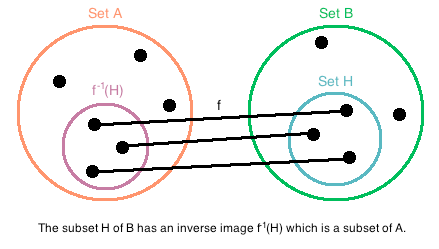
\includegraphics[scale=0.75]{inverse}
\par\end{centering}
\caption{Inverse map}
\end{figure}

We are now ready to give the rigorous definition of a random variable.
For the remainder, we will assume an underlying probability space
$(\Omega,\mathcal{F},\mathbb{P})$.
\begin{defn}
A \emph{random variable} is a function $X\colon\Omega\rightarrow\mathbb{R}$
which satisfies, for all $B\in\mathcal{B}(\mathbb{R})$,
\[
X^{-1}(B)\equiv\left\{ \omega\in\Omega\colon X(\omega)\in B\right\} \in\mathcal{F}.
\]
The Borel $\sigma$-algebra is rather large, so the above definition
is not easy to check. The following proposition makes our lives a
bit simpler.
\end{defn}
\begin{prop}
Suppose $\mathcal{G}$ generates the Borel $\sigma$-algebra (i.e.,
$\sigma(\mathcal{G})=\mathcal{B}(\mathbb{R})$). Then, $X\colon\Omega\rightarrow\mathbb{R}$
is a random variable if and only if for each generating set $G\in\mathcal{G}$,
\[
X^{-1}(G)\in\mathcal{F}.
\]
\end{prop}
\begin{proof}
We prove only the nontrivial direction. Let
\[
\mathcal{M}=\left\{ B\subset\mathbb{R}\colon X^{-1}(B)\in\mathcal{F}\right\} .
\]
By definition, we know that $\mathcal{G}\subset\mathcal{M}$. Therefore,
$\sigma(\mathcal{G})\subset\sigma(\mathcal{M})$. If $\mathcal{M}$
is a $\sigma$-algebra, it follows that
\[
\mathcal{B}(\mathbb{R})=\sigma(\mathcal{G})\subset\sigma(\mathcal{M})=\mathcal{M},
\]
as desired. To check that $\mathcal{M}$ is a $\sigma$-algebra, verify
the three properties:
\begin{enumerate}
\item $X^{-1}(\emptyset)=\emptyset\in\mathcal{F}$.
\item If $B\in\mathcal{M}$, then $X^{-1}(B^{c})=(X^{-1}(B))^{c}\in\mathcal{F}$.
\item If $B_{1},B_{2},\ldots\in\mathcal{M}$, then $X^{-1}(\cup_{n\geq1}B_{n})=\cup_{n\geq1}X^{-1}(B_{n})\in\mathcal{F}$.\qedhere
\end{enumerate}
\end{proof}
The above proposition is particularly useful when we take $\mathcal{G}$
to be the set of intervals $\mathcal{G}=\{(-\infty,x]\colon x\in\mathbb{R}\}$.
In this case...
\begin{cor}
\label{cor:simpler_measurability_criteria}$X\colon\Omega\rightarrow\mathbb{R}$
is a random variable if and only if for each $x\in\mathbb{R}$,
\[
\left\{ \omega\in\Omega\colon X(\omega)\leq x\right\} \in\mathcal{F}.
\]
\end{cor}
\begin{proof}
If $G=(-\infty,x]$,
\[
X^{-1}(G)=X^{-1}((-\infty,x])=\left\{ \omega\in\Omega\colon X(\omega)\leq x\right\} .\qedhere
\]
\end{proof}
We will often use the above corollary to prove something is a random
variable. To simplify notation, we often write
\[
\left\{ \omega\in\Omega\colon X(\omega)\leq x\right\} =\left\{ X\leq x\right\} .
\]
The above means that for a random variable $X$, $\mathbb{P}(\{X\leq x\})$
(i.e., the probability that $X$ is at most $x$) is always well-defined.
We define $\{X<x\}$, $\{X=x\}$, $\{X\geq x\}$, and $\{X>x\}$ similarly.
\begin{prop}
Let $X$ be a random variable. Then, $\{X<x\},\{X=x\},\{X\geq x\},\{X>x\}\in\mathcal{F}$.
\end{prop}
\begin{proof}
Let's just do the case of $\{X<x\}$. We can write
\[
\left\{ X<x\right\} =\bigcup_{\substack{q\in\mathbb{Q}\\
q>0
}
}\left\{ X\leq x-q\right\} ,
\]
in which case we see that $\{X<x\}$ is nothing other than a countable
union of sets of the form $\{X\leq a\}$, which we know to be in $\mathcal{F}$.
\end{proof}
%
\begin{prop}
Let $X$ and $Y$ be random variables (on a probability space $(\Omega,\mathcal{F},\mathbb{P})$)
and let $a$ be a real number. Then, the following are also random
variables:
\begin{enumerate}
\item $aX$.
\item $X+Y$.
\item $XY$.
\item $Z$ defined by $Z(\omega)=\begin{cases}
Y(\omega)/X(\omega) & \text{if }X(\omega)\neq0\\
0 & \text{if }X(\omega)=0.
\end{cases}$
\end{enumerate}
\end{prop}
\begin{proof}
Let $x\in\mathbb{R}$ be arbitrary.
\begin{enumerate}
\item Note that $\{aX\leq x\}=\{X\leq x/a\}$. Since $X$ is a random variable,
$\{X\leq x/a\}\in\mathcal{F}$.
\item It is sufficient to prove that $\{X+Y>x\}\in\mathcal{F}$ since $\{X+Y>x\}=\{X+Y\leq x\}^{c}$.
Note that
\[
\left\{ X+Y>x\right\} =\bigcup_{q\in\mathbb{Q}}\left\{ X>q\right\} \cap\left\{ Y>x-q\right\} .
\]
In this form, it is clear that $\{X+Y>x\}\in\mathcal{F}$.
\item For a real number $a$, define
\[
a^{+}=\max\{a,0\}\qquad\text{and}\qquad a^{-}=\max\{-a,0\}
\]
as its positive and negative parts. Since for any real number $a$
we have $a=a^{+}-a^{-}$, it follows that
\[
XY=\left(X^{+}-X^{-}\right)\left(Y^{+}-Y^{-}\right)=X^{+}Y^{+}+X^{+}Y^{-}-X^{-}Y^{+}+X^{-}Y^{-}.
\]
Therefore, it is sufficient to consider the case in which $X$ and
$Y$ are nonnegative. Moreover,
\[
\left\{ XY>x\right\} =\bigcup_{\substack{q\in\mathbb{Q}\\
q>0
}
}\left\{ X>q\right\} \cap\left\{ Y>x/q\right\} .
\]
\item It is sufficient to consider the case of $Y=1$ since $Y/X=Y(1/X)$.
In this case,
\begin{align*}
\left\{ Z\leq z\right\}  & =\Omega\cap\left\{ Z\leq z\right\} \\
 & =\left(\left\{ X\neq0\right\} \cup\left\{ X=0\right\} \right)\cap\left\{ Z\leq z\right\} \\
 & =\left(\left\{ X\neq0\right\} \cap\left\{ Z\leq z\right\} \right)\cup\left(\left\{ X=0\right\} \cap\left\{ Z\leq z\right\} \right)\\
 & =\left(\left\{ X\neq0\right\} \cap\left\{ 1/X\leq z\right\} \right)\cup\left(\left\{ X=0\right\} \cap\left\{ 0\leq z\right\} \right).
\end{align*}
First, note that $\{0\leq z\}$ is either equal to $\emptyset$ or
$\Omega$, and hence $\left\{ X=0\right\} \cap\left\{ 0\leq z\right\} \in\mathcal{F}$.
We leave verifying that $\left\{ X\neq0\right\} \cap\left\{ 1/X\leq z\right\} \in\mathcal{F}$
as an exercise.\qedhere
\end{enumerate}
\end{proof}

\section{Distribution functions}
\begin{defn}
The \emph{distribution function} of a random variable $X$ is the
function $F\colon\mathbb{R}\rightarrow[0,1]$ defined by
\[
F(x)=\mathbb{P}(\left\{ X\leq x\right\} ).
\]
\end{defn}
The distribution function is sometimes called the \emph{cumulative
distribution function} (CDF).
\begin{example}
Flip a coin twice. Let $X$ be the number of heads $H$ which show
up. Since
\begin{align*}
\mathbb{P}(\left\{ TT\right\} ) & =1/4\\
\mathbb{P}(\left\{ HT,TH\right\} ) & =2/4\\
\mathbb{P}(\left\{ HH\right\} ) & =1/4,
\end{align*}
we have that
\[
F(x)=\begin{cases}
0 & \text{if }x<0\\
1/4 & \text{if }x<1\\
3/4 & \text{if }x<2\\
1 & \text{if }x\geq2.
\end{cases}
\]
\end{example}
\begin{rem}
It now becomes clear why a random variable $X$ requires $\{X\leq x\}\in\mathcal{F}$!
It is so that the dstribution function is well-defined at any point
$x$.
\end{rem}
In terms of the inverse function, note that
\[
F(x)=\mathbb{P}(\,X^{-1}((-\infty,x])\,).
\]
\begin{prop}
Let $X$ be a random variable and $F$ be its distribution function.
Then,
\begin{enumerate}
\item $F$ is nondecreasing.
\item $F$ is right continuous. That is, $F(x)=\lim_{y\downarrow x}F(y)$
for each $x$.
\item $\lim_{x\rightarrow-\infty}F(x)=0$ and $\lim_{x\rightarrow\infty}F(x)=1$.
\end{enumerate}
\end{prop}
\begin{proof}
Let $A_{x}=\{X\leq x\}$ so that $F(x)=\mathbb{P}(A_{x})$.
\begin{enumerate}
\item If $x\leq y$, then $A_{x}\subset A_{y}$ and hence $\mathbb{P}(A_{x})\leq\mathbb{P}(A_{y})$.
\item Let $(y_{n})_{n}$ be a sequence converging to $x$ from above. Then,
we have $A_{y_{1}}\supset A_{y_{2}}\supset\cdots$ and hence $\lim_{n\rightarrow\infty}\mathbb{P}(A_{y_{n}})=\mathbb{P}(\cap_{n\geq1}A_{y_{n}})=\mathbb{P}(A_{x})$.
\item Note that $A_{-1}\supset A_{-2}\supset\cdots$ and hence $\lim_{n\rightarrow\infty}\mathbb{P}(A_{-n})=\mathbb{P}(\cap_{n\geq1}A_{-n})=\mathbb{P}(\emptyset)=0$.
Similarly, $A_{1}\subset A_{2}\subset\cdots$ and hence $\lim_{n\rightarrow\infty}\mathbb{P}(A_{n})=\mathbb{P}(\cup_{n\geq1}A_{n})=\mathbb{P}(\Omega)=1$.
\end{enumerate}
\end{proof}
Since $F$ is monotone, it follows that $F$ has at most countably
many discontinuities. We define
\[
F(x-)=\lim_{y\uparrow x}F(x)
\]
as the left-hand limit of $F$.

\begin{figure}
\begin{centering}
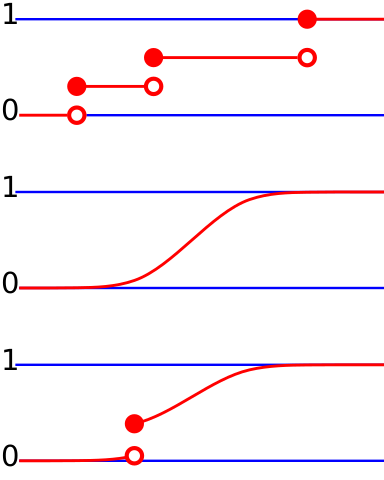
\includegraphics[scale=0.5]{cdf}
\par\end{centering}
\caption{Examples of distribution functions}
\end{figure}
\begin{prop}
Let $X$ be a random variable with distribution function $F$. Then,
\begin{enumerate}
\item $\mathbb{P}(\{X<x\})=F(x-)$.
\item $\mathbb{P}(\{X=x\})=F(x)-F(x-)$.
\item If $a<b$, $\mathbb{P}(\{a<X\leq b\})=F(b)-F(a)$.
\item $\mathbb{P}(\{X>x\})=1-F(x)$.
\end{enumerate}
\end{prop}
The above implies that if $F$ is continuous, then $\mathbb{P}(\{X=x\})=0$
for all $x$! This means that there is zero probability of any particular
realization of a random variable. Positive probability is assigned
only to ranges (e.g., $\{a<X\leq b\}$).

\section{Indicator random variables}
\begin{defn}
Let $A\in\mathcal{F}$. The \emph{indicator random variable on $A$
}is the function
\[
I_{A}(\omega)=\begin{cases}
1 & \text{if }\omega\in A\\
0 & \text{if }\omega\notin A.
\end{cases}
\]
\end{defn}
Note that for an indicator random variable $I_{A}$, we have $\mathbb{P}(\{I_{A}=1\})=\mathbb{P}(A)$
and $\mathbb{P}(\{I_{A}=0\})=\mathbb{P}(A^{c})=1-\mathbb{P}(A)$. 
\begin{example}
You play a game in which you roll a dice, and if the number you roll
is greater than four, you get \$2. Otherwise, you lose \$1. How do
we represent your winnings as a random variable?

Let $\Omega=\{1,\ldots,6\}$. Since this is a finite sample space,
we can safely take $\mathcal{F}=2^{\Omega}$ and define $\mathbb{P}$
by $\mathbb{P}(\{\omega\})=1/6$ (each outcome is equally as likely).
The random variable corresponding to your winnings is
\[
X(\omega)=2I_{\{\omega>4\}}(\omega)-I_{\{\omega\leq4\}}(\omega).
\]
We'll often express this more succinctly as
\[
X=2I_{\{\omega>4\}}-I_{\{\omega\leq4\}}.
\]
\end{example}
\begin{rem}
There are many other common notations for indicator functions. It
helps to be aware of these:
\[
I_{A}(\omega)\equiv\mathbf{1}_{A}(\omega)\equiv\chi_{A}(\omega)\equiv[A](\omega).
\]
\end{rem}

\section{Borel measurable functions}

In closing this section, we introduce the notion of a Borel measurable
function, which will give us our final piece of insight as to why
we care about Borel $\sigma$-algebras.
\begin{defn}
We say $f\colon\mathbb{R}\rightarrow\mathbb{R}$ is a \emph{Borel
measurable function} (a.k.a. Borel function) if for each $B\in\mathcal{B}(\mathbb{R})$,
\[
f^{-1}(B)\in\mathcal{B}(\mathbb{R}).
\]
That is, the inverse image of a Borel set is also a Borel set.
\end{defn}
\begin{prop}
If $f\colon\mathbb{R}\rightarrow\mathbb{R}$ is continuous, it is
Borel measurable.
\end{prop}
\begin{proof}
Let
\[
\mathcal{M}=\left\{ B\subset\mathbb{R}\colon f^{-1}(B)\in\mathcal{B}(\mathbb{R})\right\} .
\]
As usual, we can show that $\mathcal{M}$ is a $\sigma$-algebra (check).
Let $\mathcal{G}$ be the set of open intervals in $\mathbb{R}$.
Then, since $f$ is continuous, $\mathcal{G}\subset\mathcal{M}$ and
as such, $\mathcal{B}(\mathbb{R})=\sigma(\mathcal{G})\subset\sigma(\mathcal{M})=\mathcal{M}$
as desired.
\end{proof}
\begin{xca}
Let $X$ be a random variable and $f\colon\mathbb{R}\rightarrow\mathbb{R}$
be a Boreal measurable function. Show that $Y$ defined by $Y(\omega)=f(X(\omega))$
is a random variable.
\end{xca}
The above implies, most importantly, that taking the composition of
a continuous function $f$ and a random variable $X$ yields a new
random variable.
\end{document}
